%-----------------------------------------------------------------------------
%
%               Template for sigplanconf LaTeX Class
%
% Name:         sigplanconf-template.tex
%
% Purpose:      A template for sigplanconf.cls, which is a LaTeX 2e class
%               file for SIGPLAN conference proceedings.
%
% Author:       Paul C. Anagnostopoulos
%               Windfall Software
%               978 371-2316
%               paul@windfall.com
%
% Created:      15 February 2005
%
%-----------------------------------------------------------------------------


\documentclass[preprint,nocopyrightspace]{styles/sigplanconf}

% The following \documentclass options may be useful:
%
% 10pt          To set in 10-point type instead of 9-point.
% 11pt          To set in 11-point type instead of 9-point.
% authoryear    To obtain author/year citation style instead of numeric.

\usepackage{amsmath}
\usepackage{times}
\usepackage{epsfig}
\usepackage{subfigure}
\usepackage{balance}
\usepackage{color}
\usepackage{mdwlist}
\usepackage{fancyvrb}
\usepackage{graphicx}

\newcommand{\kimsays}[1]{{\tiny{\bf\color{red} KIM SAYS: #1}}}

\begin{document}

\conferenceinfo{PPoPP 2011}{February 12-16, 2011, San Antonio, TX} 
\copyrightyear{2010} 
\copyrightdata{[to be supplied]} 

\titlebanner{Submitted to PPoPP 2011. Please do not distribute.} % These are ignored unless
\preprintfooter{A Language and Optimizing Compiler for Iterative Stencil Loops}   % 'preprint' option specified.

\title{\vskip-0.1in{}A Language and Optimizing Compiler for Iterative Stencil Loops \\[-0.55in]}
%\title{A Language and Optimizing Compiler for Iterative Stencil Loops}
%\subtitle{Subtitle Text, if any}

\authorinfo{}{}{}
%\authorinfo{Gregory Faust, Salvatore Valente, Kevin Skadron, and Kim Hazelwood}
%           {Computer Science Department, University of Virginia}
%           {\{gf4ea,sv9wn,skadron,hazelwood\}@cs.virginia.edu}

\maketitle

\begin{abstract}

Parallel hardware is now widely available, yet writing and optimizing
parallel programs using sequential languages is difficult and error prone.
Therefore, it is useful to consider new language constructs that make it easier
for programmers to express parallel applications without the need to attend to
all the complexity of writing parallel algorithms.  Here we present a new
language in which users can easily express computations that involve iterative
stencil calculations.  Such computations form an important subset of parallel
algorithms and are widely used in scientific, engineering, and other important
application areas.

Specifically, we present a novel high-level language called Stencil Language
(SL).  Using SL, a programmer need only express the central kernel of their
computation, not an entire parallel program.  We have also built a
translator for SL capable of translating the SL program into code for different
parallel programming models.  We provide an initial translation into optimized
code for the C++ extensions of the CUDA programming model for NVIDIA GPUs.  Our
CUDA optimizer is an extension of a previously proposed analytical model for
CUDA stencil applications.  Our model improves over the previous model by
automatically utilizing both static and dynamic information about the
application and the specific GPU environment in which the application is
running.  This allows the optimized version of the application to be derived
without the need for the application developer to specify any execution
environment specific information.  Finally, we provide results that show that
the code generated from SL for CUDA is up to 2.3X faster than na\"{i}ve CUDA code
across six applications and two generations of NVIDIA hardware.

\end{abstract}

%\category{CR-number}{subcategory}{third-level}
%\terms term1, term2
%\keywords keyword1, keyword2

\section{Introduction}

{\em Iterative stencil loops} (ISLs)~\cite{li} are a class of loops that are
commonly used in fields including numerical simulations and signal processing.
Such loops compute a time varying set of values in an array.  The value for
each array element in each time step depends upon the value for that element
and its nearby neighboring elements from the previous time step.  
The pattern of the accessed neighboring elements is called the {\em stencil}.
This access pattern means that each element in the current time step 
can be calculated independently of all others.  
Therefore, techniques that take advantage of data
parallelism are applicable to ISLs, and can often lead to dramatic speedups
over serialized implementations.  Yet, such data parallel implementations of
ISLs present several challenges.

A typical implementation of an ISL on parallel hardware will divide the array
into subsections called {\em tiles} and assign one or more tiles to each
processor.  A complication of this technique is that the neighboring elements
near the edge of a tile assigned to one processor may reside in a
tile assigned to another processor.  Therefore, a certain amount of data
sharing between the separate tiles assigned to different processors is required.
Furthermore, on architectures where the cost of data communication between
processors is expensive, an optimal ISL implementation will allow each
processor to calculate several time steps for its tile(s) before communicating
with other processors.

To accommodate this communication delay, the tiles assigned to different 
processors must now overlap.
The amount of overlap increases with the number of time steps
between communication events.  
In addition, values of array elements in the overlap area must 
be redundantly calculated because each processor needs the boundary values 
locally for the intermediate time steps.
On such hardware, the correct number of time steps to
allow between processor synchronization is therefore a trade-off between the
costs of the synchronization and associated data exchange, and the number of
redundant values that are calculated.  

These trade-offs are poorly understood and are highly architecture dependent.  
They are particularly challenging on new accelerator processors with novel 
memory hierarchies and synchronization support.
GPUs are one prominent example.  
They have attracted great interest for general-purpose engineering and scientific
computing due to their high data-parallel throughput and low cost.

What is needed is a way for users to express ISL computation in a
way that allows them to focus on their application, and not on the parallel
optimization techniques needed for fast performance.  In this paper, we discuss
our efforts to provide such a system.  Our contributions are as follows:

\begin{itemize*}
\item We have defined a {\em stencil language} called SL.
  This is a formal high-level language in which a programmer can describe 
  an ISL computation.  
  By design, a description written in the language must
  include all of the information necessary to calculate the correct
  results, and none of the information that would tie its performance
  to a particular architecture.
\item We have created a front-end compiler for SL that can be extended with
  multiple back-ends.  Based on a single source file, it could output
  efficient code for a variety of parallel architectures including
  CUDA~\cite{CUDA1, CUDA2}, OpenCL~\cite{OpenCL}, OpenMP~\cite{OpenMP}, 
  or pthreads~\cite{pthreads}.
\item We have provided an initial back-end for NVIDIA GPUs through 
  source-to-source translation to their CUDA programming environment.
\item
  Our CUDA code optimizer transparently calculates the optimal tile size and 
  time steps between synchronization, and takes advantage of scratchpad memory.
  It extends the analytical model proposed by Meng and Skadron~\cite{meng}.
\item
  Our system automatically collects all the necessary application specific 
  and execution environment information needed by the model.  
  Some is derived statically from the SL program, and the rest is derived dynamically at runtime.
\item Dynamic acquisition of the execution environment information 
  allows the generated code to calculate good values on a variety 
  of GPU cards.
  We demonstrate this capability by using our optimizer developed on the 
  GT200 series of GPUs on the newer Fermi architecture.
\end{itemize*}

The remainder of this paper is organized as follows.  We first provide a high
level overview of our system in Section 2, describing the various components
and their information flow.  Then, in Section 3, we define the ISL terminology
necessary for understanding the details of our SL language and compiler, which
are then presented in Sections 4 and 5, respectively.  Section 6 discusses the
optimized CUDA code that is generated by our compiler, and Section 7 presents
the performance of that generated code.  Section 8 compares our approach to
prior work, while Section 9 concludes and discusses our plans for future work.

\section{SL System Organization}

Figure~\ref{fig:SysOrg} shows the system organization of the SL compiler,
and the information flow in a typical scenario.  
The application programmer specifies their ISL computation in an SL source
file.  The remainder of their application is specified in C or C++.  
In a simple scenario, the application code will set up the array upon which
the ISL will operate, and call the code generated by the SL compiler to do
the actual ISL computation.  The results of the ISL computation can then be
used by the application as necessary.  The SL compiler generates a C Header File 
for inclusion in the application code to declare the signature of the ISL
subroutine(s).

The SL compiler takes in two sources of information.  One is the SL source file
that specifies the user's ISL computation.  In addition, the SL system 
contains a template library that includes hand optimized implementations of 
the general structure of an ISL computation for various runtime environments.
These templates are written by the SL system developers, not the SL user.
Based on the user specified target environment, the SL compiler selects the
appropriate library template and modifies it to implement the user's particular
stencil calculation.  The SL compiler outputs the modified template as C source code.
The SL generated C source and the user's application C source are each compiled and
linked together into a final executable.

While the simple case shows a single SL computation in an application, many
scientific applications may contain more than one ISL computation in a pipeline.
This usage scenario is supported by our architecture.  Each ISL computation
is specified in its own SL source file.  The user's application code can then
call the generated subroutine for each ISL computation in sequence, passing the results
of one calculation as input into the next.

While Figure~\ref{fig:SysOrg} shows the general system organization, to date
the template library only contains optimized templates for the CUDA
environment.  These templates include the analytical model for estimating the
runtime for the generated CUDA kernel, plus the code to dynamically
gather the runtime environment specific information needed by the model, and
finally calculate the optimal tile size and time steps between
synchronizations.
The CUDA template causes the SL compiler to generate CUDA source
code (a .cu file) which is then fed into NVIDIA's NVCC compiler driver.

\begin{figure}
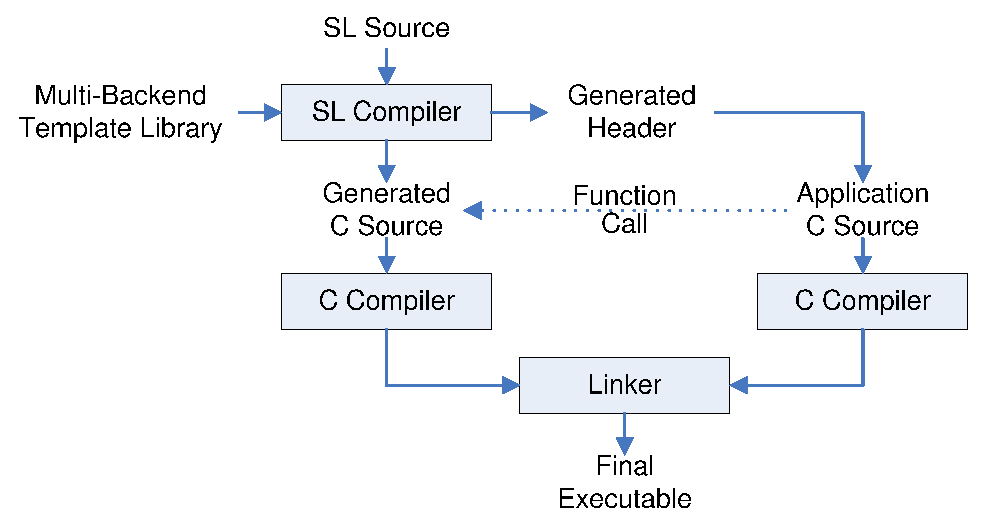
\includegraphics[clip,trim=1.0in 6.4in 1.0in 1.0in,width=3.3in]{figures/WorkFlow}
\caption{SL System Diagram showing information flow in a typical usage scenario.
The SL source is combined by the SL compiler with the appropriate optimized back-end
template. The resultant generated C subroutine for the ISL calculation
is called by the rest of the user's application code written in C or C++.}
\label{fig:SysOrg}
\end{figure}

\section{Iterative Stencil Loops: Terms \& Background}

{\em Iterative stencil loops} (ISLs)~\cite{li} are a class of loops
commonly used in numerical simulations and
signal processing.  ISLs usually operate on matrices with one, two, or
three dimensions.  An ISL calculation takes an input matrix $m_{in}$
and produces an output matrix $m_{out}$.  The calculation has the
following properties:

\begin{enumerate*}
\item $m_{in}$ and $m_{out}$ have the same number of dimensions and
  are the same size.
\item Each value in $m_{out}$ is calculated independently of each
  other value in $m_{out}$.
\item There is a single function which is used to calculate each value
  in $m_{out}$ regardless of the coordinates of the value.
\end{enumerate*}

For example, suppose $m_{in}$ is a two-dimensional matrix, and the stencil calculation 
is defined as ``$m_{out}[x, y] =$ the average
of the north, south, east, and west neighbors of $m_{in}[x, y]$''.
Then this function will be calculated for every cell in $m_{out}$.

The {\em stencil} is the set of cells in the input matrix that is used in the stencil calculation, relative to
the coordinates of the cell that is being calculated. 
In the above example, the stencil is a set
of four cells: the north, south, east, and west neighbors.

The process of calculating a complete output matrix is called an {\em
  iteration} or a {\em time step}.  At the end of an iteration, 
the output matrix $m_{out}$ is used as the input matrix to the
next iteration.  This loop can continue for as long as necessary.
Some iterative stencil loops are defined to run for a predetermined
number of time steps, while others are defined to run until
the values converge.

Stencil calculations are data parallel.  Since each value in
a time step is calculated independently of each other, the values can be
calculated in any order or at the same time.  If the matrix has $n$
cells and the computer has $k$ {\em processing elements} (PEs) available,
then each processor only needs to calculate a block of size $n/k$.  This
partitioning of the matrices among multiple processors is called
{\em tiling}, and the block calculated by a PE is called a
{\em tile}.

When a PE calculates a given tile for many iterations, that PE can
take advantage of both spatial locality and temporal locality.
\begin{itemize*}
\item {\bf Spatial locality.} As a general rule, stencil calculations
  use each input value multiple times.  For example, say the
  stencil is defined as the cell's left and right neighbors.  When a
  PE calculates the cell value at $x=i$, it reads that value of
  the right neighbor at $x=i+1$.  Then, when it calculates the
  cell value at $x=i+2$, it reads the left neighbor, which
  is the value at $x=i+1$ again.  Thus, a PE can optimize this
  computation by keeping input values in a local cache or scratchpad.
\item {\bf Temporal locality.} If a PE generates an output value
  during iteration $t$, then that PE can use that value as an input
  value during iteration $t+1$.
\end{itemize*}

Unfortunately, if each PE is given only those array values that fall within its
tile size, cells along the boundary of the tile cannot find all of their input
values in the local processor cache.  These cells must obtain some of their
input values from array values in adjacent tiles assigned to other PEs.  In the
example above, the cell in the bottom left corner of a tile will require values
for both its south and west neighbors from neighboring tiles.  The region of
data surrounding a tile that is needed from adjacent tiles is called its {\em
ghost zone} or GZ.

In addition, in order to take advantage of temporal locality, each PE may want
to compute more than one time interval with the array values it has stored
locally.  However, at each successive time interval, more and more values at
the periphery of the PEs local store will become stale.  For example, consider
the 2D tile computation shown in Figure~\ref{fig:trapezoid}(a).  It shows the
shrinking number of valid values calculated in a tile over four time intervals.
In the first time interval $i$, with a stencil size of one, the PE will require
a GZ of size one all around the periphery of the tile.  However, in calculating
the second time interval $i+1$, the values in the original GZ are still from
time $i$ and are now out of date.  Therefore, the PE is only able to calculate
a smaller number of valid values, and the size of the GZ has expanded by the
size of the stencil on all sides of the tile.  In the diagram, this progression
of stale values and expanding GZs will continue inward through time interval
$t+3$, after which only the inner most rectangle will have valid values.

\begin{figure}
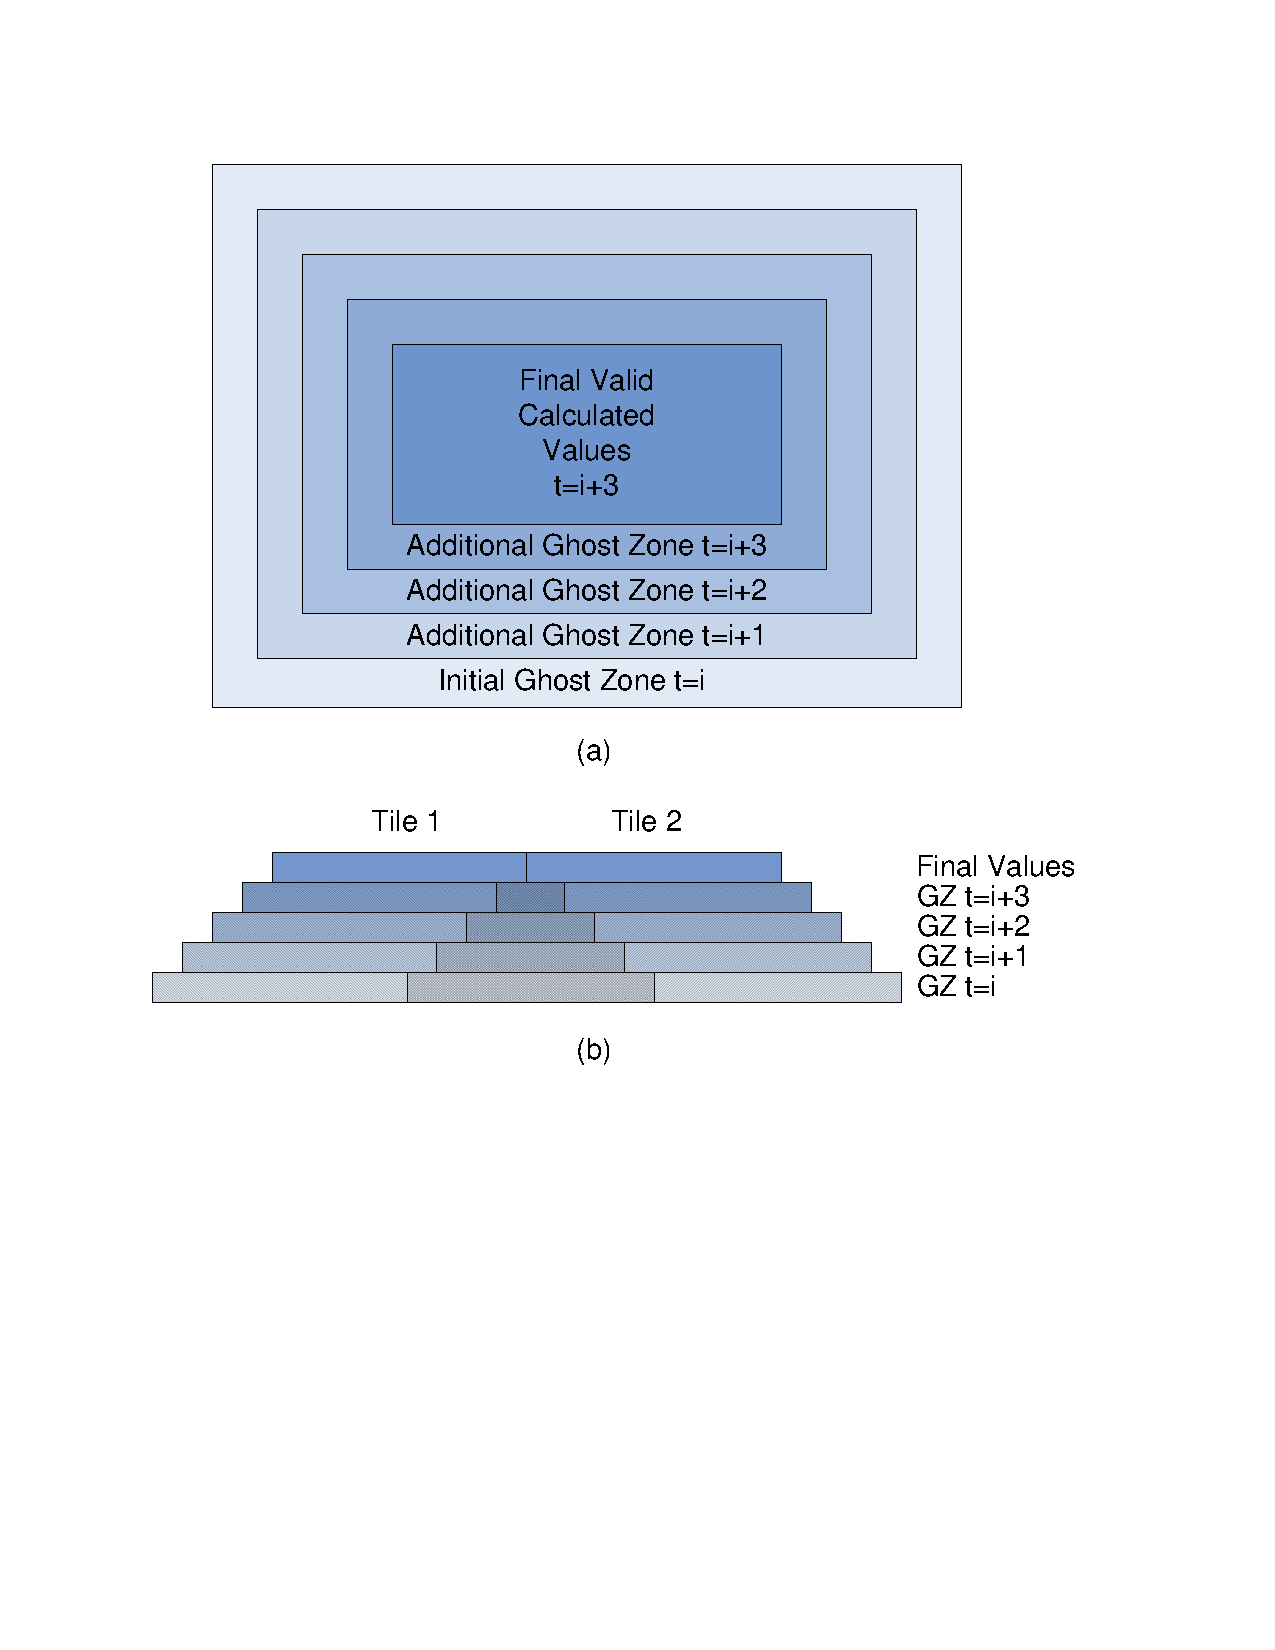
\includegraphics[clip,trim=1.0in 3.5in 1.3in 1.0in,width=3.3in]{figures/Diagrams}
\caption{(a) For a single tile in a 2D matrix, the number of valid calculated
values decreases with each additional time interval calculated between 
synchronization events.  After 4 time steps, only the inner most rectangle
of $n$ values are valid.  (b)  Two adjacent tiles shown from the plane of the 2D array
with time in the vertical dimension.  In the first time step 
(diagram bottom) there is substantial overlap in the ghost
zones in order to have the resultant valid values just abut after 4 time steps 
(diagram top).}
\label{fig:trapezoid}
\end{figure}

Figure~\ref{fig:trapezoid}(b) shows the overlap in GZs between two adjacent
tiles for the same computation over four time intervals with time now shown in
the vertical dimension.  Each PE must start with GZ of size four in order to
have valid values computed for the resultant tiles cover the entire input
array.  Because the size of the area of valid values for a PE shrink with time
in this way, the number of time intervals each PE calculates between
synchronization events is called the {\em pyramid height} or PH of the ISL.  In
general, the size of the required GZ is equal to twice the size of the stencil
times the PH.  In addition, the values for cells in all but the initial GZ are
redundantly calculated by adjacent PEs.

As a result of the required data exchange between PEs described above, ISL
algorithms may spend considerable time stalled due to communication and
synchronization delays.  Because synchronization events can have high
latencies, it is often better to reduce the number of synchronizations between
PEs by increasing the PH and therefore the size of the GZ.  However, as we have
seen, larger GZs result in larger data exchanges at each synchronization, and
also lead to redundant cell value calculations.  Therefore, the choice of the optimal PH
for an ISL is a trade-off between these two competing costs/benefits.  Yet, the
performance of ISLs depends critically upon the correct choice.  Therefore, 
there have been several attempts to optimize these trade offs, such as the 
study by Meng and Skadron~\cite{meng} in which they examined the
problem of writing efficient ISL code in the CUDA language to run on an NVIDIA
GPU.  They defined a mathematical model for calculating the optimal PH for an
ISL targeted for that runtime environment.  We have built upon the results of that
study, and have fully automated that optimization process in our SL compiler, 
as we demonstrate in the following sections. 

\section{Stencil Language Definition}

Figure~\ref{fig:hotspot} shows an SL description of the ``Hotspot''
calculation.  This code calculates the temperature patterns in a
two-dimensional microchip where the current state is a function of the previous
state, the edge values, and a 2D read-only ``power usage'' matrix.
We will examine the various aspects of this example in turn.

\begin{figure}
\begin{footnotesize}
\begin{verbatim}
NumDimensions 2
StencilSize (1, 1)
DataType float
FunctionName runHotspot

ScalarVariables (
  float Rx, float Ry, float Rz
}
CellValue {
  float pvalue, value, term1, term2, term3, sum;
  pvalue = read(y * input_size.x + x);
  value = get(0, 0);
  term1 = (get(0, 1) + get(0, -1) - value) / Ry;
  term2 = (get(1, 0) + get(-1, 0) - value) / Rx;
  term3 = (80.0 - value) / Rz;
  sum = pvalue + term1 + term2 + term3;
  return(value + sum);
}
EdgeValue {
  return value;
}
\end{verbatim}
\end{footnotesize}
\caption{The Hotspot.sl stencil language file.  This example
  shows a 2D stencil calculation where
  each cell value is based on the values of that cell's
  immediate neighbors.  The read-only data is interpreted as a
  2D matrix in row-major order which indicates 
  that some areas of the chip inherently run hotter then other areas.}
\label{fig:hotspot} 
\end{figure}

\subsection{Syntax}

A stencil language file is a text file that
contains a set of key-value pairs.
A key is an alphanumeric string.  A value can be:
\begin{itemize*}
\item an integer
\item a name comprised of alphanumeric and underscore characters
\item a list of names, inside parentheses, separated by commas
\item a block of C code inside of curly braces
\end{itemize*}

\subsection{Content}

The currently supported SL keywords are as follows.

\begin{itemize}
\item {\bf NumDimensions} -- A stencil may have 1, 2, or 3 dimensions.
\item {\bf StencilSize} -- The size of the stencil in each dimension.
  If the stencil size is 1 in the $x$ dimension, then the value of the
  cell at $(x, y)$ may be based on the previous iteration's values of
  the cells in the $x-1$ and $x+1$ coordinates.
\item {\bf DataType} -- The data may be 32 bit or 64 bit integers or
  floating-point numbers.  The values are {\tt int}, {\tt int64}, {\tt
    float}, and {\tt double}.  Values may be signed or unsigned.
\item {\bf FunctionName} -- The name of the function that will be exported
  from the generated source file.  The first argument to the function,
  {\tt data}, will be a matrix of the specified data type with the
  specified number of dimensions.  As input to the function, {\tt
    data} must contain the initial state of the problem.  It must
  contain valid data in each cell.  As
  output from the function, it will contain the final data.  The next
  $n$ arguments to the function are the input sizes in each dimension.
  The next argument is the number of iterations to run.
\item {\bf ScalarVariables} -- A list of numeric variables that will
  be arguments to the exported function after {\tt data, x, y, z,
    iterations}.  The caller will pass these arguments to the
  function, and then the stencil calculator will be able to use these
  variables (read-only) in its calculations.
\item {\bf CellValue} -- A block of C code that will be run for every
  cell in the data set in every iteration.  The code has access to the
  following variables and functions:
\begin{itemize}
\item {\tt x, y, z} -- Coordinates of current cell in each dimension.
\item {\tt iteration} -- Iteration number.  Iteration 0 is
  given as input, so this code will first be called with {\tt iteration}=1.
\item {\tt input\_size} -- a structure with {\tt x}, {\tt y}, and {\tt
  z} fields, containing the total size of the input
\item All variables listed in the {\bf ScalarVariables} field.
\item {\tt get(...)} -- a function that efficiently returns values
  from the stencil from the previous iteration.  The parameters are
  relative to the current cell.  For example, in a 2D
  stencil, the west and east neighbors can be retrieved with {\tt
    get(-1, 0)} and {\tt get(1, 0)}.
\item {\tt read(...)} -- a function to access read-only data (see below).
\end{itemize}
The block of code returns the new cell value.
\item {\bf EdgeValue} -- A block of C code that returns the cell value
  of cells that are outside the bounds of the input.  This code has
  access to the same variables as the {\bf CellValue} code.  Note that
  at least one of {\tt x}, {\tt y}, or {\tt z} will be out of bounds
  -- it will be either less than zero or greater than or equal to the
  size of that dimension.  This code may not use the {\tt get()}
  function.  Instead, it can access the {\tt value} variable, which
  will contain the value of the nearest cell in bounds from the
  previous iteration.
\end{itemize}

\subsection{Read Only Data}

The generated source file will export two functions.  One of the
functions will have the given function name.  The other function will
have the function name appended with {\tt SetData}.  For example, if
the stencil language file says:
\begin{verbatim}
FunctionName runStencil
\end{verbatim}
then the generated source file will export these two functions:
\begin{itemize*}
\item {\tt runStencil()}
\item {\tt runStencilSetData()}
\end{itemize*}

\noindent The SetData function takes two arguments:
\begin{enumerate*}
\item An array of elements of the specified data type
\item The number of elements in the array
\end{enumerate*}
If a program calls {\tt runStencilSetData()} with an
array, and then calls {\tt runStencil()}, then the stencil
calculator will have read-only access to this data in the array.  The
{\bf CellValue} code can access the $i$th read-only data element by
calling {\tt read(i)}.


\section{Stencil Language Compiler}

We implemented the stencil language compiler in fewer than 600 lines of
Java code.  The compiler operates as follows:
\begin{enumerate*}
\item Converts a stencil language file into a token stream
\item Parses the token stream into a symbol table
\item Reads a plain text template file
\item Outputs a new file which contains the template integrated with
  the stencil description
\end{enumerate*}

Step 1 is implemented by {\tt Tokenizer.getToken()}.  A token is
either a string of alphanumeric characters or any symbol token that is
in the language such as parentheses, commas, etc.  Also, the tokenizer
can recognize comments and blocks of C code.

Step 2 is implemented by {\tt Stencil.parse()}.  It runs a loop that
reads a key and then parses a value, which may be an integer, a
string, a list, or a block.  The parser verifies that the key is
defined by the language and that the value has the right type for that
key, and then it adds the key value pair to a symbol table.

Step 3 is implemented by the creator method of the {\tt Template}
class.  It stores the template text in the Template instance.

Step 4 is implemented by {\tt applySymbolTable()} method.  It looks
for instances of {\tt @name@} in the text.  For each instance that it
finds, it looks up {\tt name} in the symbol table, and it replaces the
variable with the value.

This design can easily support multiple architectures
and optimizations.  We have written templates for CUDA code for 1D,
2D, and 3D stencil calculations.  These templates are written such
that the {\bf CellValue} code can be dropped-in unmodified.  The 
template code is optimized for shared memory usage, and it
calculates the optimal PH.  
We have also written a template that does not use 
shared memory or GZs to compare
its performance as a na\"{i}ve CUDA implementation
to that of the optimized templates.

We are confident that an OpenMP template could be written without
changes to either the stencil language or the compiler.

\section{Generated CUDA Code}

The following subsections describe the CUDA architecture, and the 
details of the SL CUDA template and optimizer.

\subsection{CUDA Architecture Overview}

The CUDA programming model~\cite{CUDA1, CUDA2}
is a set of extensions to C++ that
NVIDIA Corporation created to allow 
their graphics cards (GPUs) to be used for general-purpose parallel 
computing.
The overall architecture of a NVIDIA GPU~\cite{Fermi} 
is shown in Figure~\ref{fig:CUDAOrg}.
The model involves using the GPU as a co-processor for the CPU.
A control thread on the CPU does some of the work for the application, 
but can call on the GPU to perform certain parallel calculations
when desired.  
The parcel of work for the GPU is called a {\em kernel}
and usually represents an inner loop that exhibits large degrees of
data parallelism.  The code for the kernel is written for one thread
as if it were the only thread running, except that it is given a
thread-id from which it can compute its position in the collection of
threads launched in the kernel invocation.  While the kernel code can
be written rather simply for simple applications, the optimal use of the
GPUs resources requires much more effort and complexity.

One source of the complexity for optimizing kernels comes from the
specialized memory hierarchy on the device due to its primary use as a graphics
accelerator.  The hardware of the GPU is organized into a collection of PEs
each of which is a SIMD core with 8 scalar processing elements.  
Both the organization of the GPU into separate PEs, and the related variety of
different types of memory, are made visible to the kernel writer.

\begin{figure}
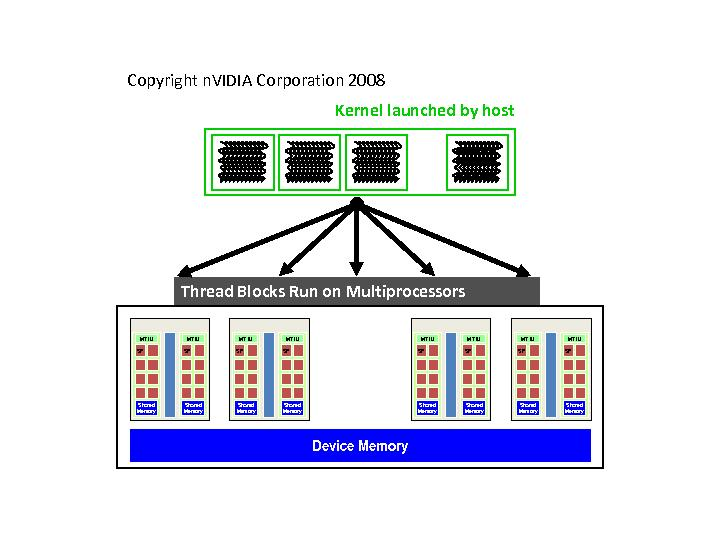
\includegraphics[clip,trim=1.4in 0.6in 1.4in 1.0in,width=3.3in]{figures/CUDADiagram}
\caption{NVIDIA GPU Diagram.  
The CPU control thread launches a kernel
with many threads per thread block.
Each thread block is assigned to a Multiprocessor (PE) containing
8 scalar processing elements and a local shared memory.
The Device Memory is global to all thread blocks and in pre-Fermi
GPUs is uncached.}
\label{fig:CUDAOrg}
\end{figure}

When calling a kernel, the user must specify the organization of the resultant
threads into thread blocks, including the 3D shape of the thread
block.  GT200 series and earlier GPU cards support up to 512 threads per block.
A thread block will be allocated by the CUDA runtime system to a particular PE
on which it will execute.  To minimize SIMD overhead, these threads are
collected into smaller groups called {\em warps}.  Each PE has a modest amount
of very fast programmer controlled scratchpad memory that NVIDIA calls {\em
shared memory} that can be shared by threads in a thread block, but  cannot be
accessed by any other thread blocks.  For the purposes of this paper, the only
other memory structure available to threads running on the GPU is a large
global memory accessible by all threads on the device.  However, on pre-Fermi
GPUs, this large memory is not cached, and has access latencies of 400
to 600 clock cycles.  Therefore, a critical optimization for kernel
writers is to properly group threads into blocks that can use the shared memory
effectively.

In addition, the CUDA model does not support any global synchronization primitive
between thread blocks during a kernel execution.  Instead, global synchronization
events require the completion of all running thread blocks and a return of control to 
the CPU control thread.  A further complication is that no data stored in the 
shared memory of a PE is persistent across kernel calls.
Such global synchronization events are therefore very costly.

The implication of this model for stencil applications is that the kernel
author must be intimately familiar with the details of the CUDA runtime
system in order to organize work units into thread blocks in such a way
that usage of shared memory is maximized, and accesses to global memory
are minimized.  Key decisions in this allocation are precisely the
tile size and PH of the stencil calculation that the optimization
model is designed to make.  In order to accurately make such decisions, it must
be able to predict the latencies of the various operations involved in the kernel's
calculations, and memory accesses on the GPU device upon with the application will run.

\subsection{SL CUDA Template}

In this section, we describe how our CUDA template code works.  
This template code is hand-written by the implementors of the SL 
system, and does not contain any application specific code.  
The application specific code from the SL specification is then
automatically merged into the template during the SL compilation
process to generate the final ISL code.  The CUDA execution
model involves both a control thread on the CPU and kernel code
that is run by many threads on the GPU.
Therefore, the CUDA template code includes both the CPU and GPU
code needed to support the application specific code provided by SL.

The primary function in the template is a C function for the CPU control
thread.  First, it calculates the tile size and the PH.  
Then, it copies the input matrix from system memory into GPU
memory.  
If an array of read-only data is used, it also
copies that data into GPU memory.
Finally, it runs a loop in which it invokes the CUDA kernel
to calculate the output matrix from the input matrix.  It runs this
loop for the specified number of iterations, divided by the PH.

Each tile is processed by one CUDA thread block, and each cell in the tile
is owned by a single thread.  The input tile size will include GZ cells.
The output tile size will be smaller.  The actual tile size used is
determined at application runtime using dynamically gathered information about
the execution environment.  For concreteness, consider a pre-Fermi
CUDA card that supports up to 512 threads per thread block.  In this case,
the 3D input tile will be $8 \times 8 \times 8$, the 2D tile $22 \times 22$,
and the 1D tile 512 cells long.  

The generated CUDA kernel includes both template code and application specific
code.  It operates as follows.  The thread calculates the $(x, y, z)$
coordinates of the cell in the matrix that it owns.  It copies that cell's
value from the input matrix into the thread block's shared memory.  After each
value has been copied into shared memory, the threads that own cells in the
outermost GZ sleep.  Those threads have completed their work.  Each other
thread calculates the new value for its cell.  For each cell in its stencil,
the thread gets the cell value from shared memory.

If the PH is greater than one, then the threads continue running.  Each thread
copies the value that it just computed into shared memory.  Then, the threads
in the second outermost GZ sleep.  Their local copies of the neighboring
cell values in the outermost GZ are now out-of-date as their values
were calculated in an adjacent tile (see Figure~\ref{fig:trapezoid}).  The
remaining threads calculate new values.  This process continues for the number
of iterations specified by PH.

When this process is complete, if a thread owned a cell that was not
in the GZ, then that cell copies the final value into device
memory.  If a thread owned a cell that was in the GZ, then
that thread does not need to do anything, since we are guaranteed that
some thread in some other thread block owned that same cell as
part of its output tile, and that
other thread will own the responsibility to write the value into
device memory.

Inside of the CUDA kernel, the program calls the user-specified
CellValue code to calculate new cell values, and it calls the
user-specified EdgeValue code to get stencil values for cells along
the edges of the matrix.  All of the remainder of the kernel code is
included in the template in the SL template library.

\subsection{Pyramid Height Calculation}

As mentioned earlier, the performance of stencil applications on parallel
hardware is critically dependent on the proper relationship between tile size
and GZ size or PH.  To calculate the optimal PH, we extended and automated the
CUDA analytical model written by Meng and Skadron.  They developed
a complex analytical model in MatLab that uses information from several sources to
calculate the expected program runtime (in GPU clock cycles).  Their
model requires several pieces of information as input.

First, it needs information about the stencil
application itself.  Some information is static such as the 
data dimensionality, the stencil size (GZ), the number of global
memory accesses required during movement of tile data into shared memory, and
the number of global accesses for read-only data required during each cell
calculation.  Other information is dynamic such as the data set size and
the number of instructions that each thread must execute (1)~in the shared
memory setup portion of the kernel, and (2)~in the kernel cell calculation.
Since they proposed but did not implement any code annotations for the stencil
applications, many of the application specific parameters were hand coded in
MatLab for the four particular test case applications.
In addition, the instruction count was gathered using
the CUDA profiler on hand-coded implementations of the test applications, and
fed to the model by hand.

Second, the specific properties of the target GPU are important.  
This includes the number of PEs, 
the number of concurrent blocks that can run on a PE, the number of threads allowed per block (tile), 
the time required for the GPU to perform a global synchronization, 
and several GPU memory performance parameters.  
These values were acquired from a number of means including hand coding some parameters 
based on the published characteristics of a few specific models of GPU, 
and some by data regression (curve fitting) of runtimes from specific applications.

We have modified and/or improved this model in several important ways.  
First, we ported the model from MatLab to C++ to include it in the application 
and perform the optimization at runtime.  
This allows gathering runtime information about the program in 
the current execution environment allowing it to be  
run on different GPUs without recompilation. 
The resulting code is better optimized for the specific characteristics of the particular hardware, 
not just the architectural features of the hardware.  While this means that the time 
to perform the optimizations is included in the total runtime for the program, the difference 
in runtimes for the wrong optimizations will generally dwarf any cost of calculating the 
optimizations themselves.  In addition, stencil applications typically take many 
iterations to converge, allowing more runtime over which to amortize the optimization costs.

Second, the static and architecture-independent application specific information about the 
dimensions of the data space, the stencil size, etc. now come directly from the SL program specification.  
These are compiled into the generated code for the ISL calculation.

Third, the remaining application-specific information is acquired dynamically at runtime.  
This includes the data set size, and the parameters that previously came from profiling 
such as the kernel thread setup time and cell value calculation time.  The latter two 
numbers are acquired by running the application with PH of 1 and 2. From these numbers, 
the setup and cell calculation times are easily computed.  Currently we throw away the 
application computation performed during these data gathering runs, but 
in the future, the time spent gathering this information could result in the 
completion of the first three iterations of the computation.

Fourth, the GPU device information is gathered through calls
to various functions provided in the CUDA runtime libraries.  In particular, we can acquire 
the number of PEs, the concurrent blocks per PE, and the maximum number of threads  
per block.  We can also query the CUDA runtime system for the number of 
threads per block for the actual kernel of the running application.  This can sometimes result in 
tighter restrictions on the allowed threads per block if, for example, the kernel requires 
more resources from the device than it can provide at the architecture maximum number of threads per block.  
This is particularly true for CUDA kernels that use a lot of registers.  
Knowing this number is critical to the optimization
because on the CUDA architecture, stencil applications generally
run faster with a larger tile size as long as the data set size is 
large enough to saturate the number of available PEs.  
Since the thread per block count determines the tile size, 
knowing this number precisely allows the optimizer to pick the largest tile size that the current GPU can handle.
Future GPUs may allow the number of threads per block to increase beyond 512.  
For example, Fermi GPUs now allow 1024 threads per block.
Gathering this information at run time
allows generated code to calculate the optimal tile size for such cards without recompilation.

Fifth, the time required for a global synchronization is acquired by running a
null kernel on the device with the same data set size parameters as are
required to run the actual kernel.

Finally, Meng and Skadron originally did a manual gradient descent on runtimes to determine 
the best PH and tile size.  Since we can determine the best tile size as described earlier, 
we do an automatic gradient descent starting at PH of 1, 
and continue calculating the model latency until it is higher than the previous one, 
then use that PH for the remainder of the application iterations.

\section{Experimental Results}

Our primary emphases are the definition of a stencil language, 
providing a compiler for it,
and optimizing the generated programs in terms of
GPU shared memory, tile size, and PH with an extension of the analytical model
of Meng and Skadron.  Therefore, we first present the results for NVIDIA's
GT200 series cards, which is the architecture for which their
performance model was developed.  The recent release of NVIDIA's Fermi series
cards presented an opportunity to test the robustness to architectural changes
of our model enhancement which utilizes dynamically-collected
information about the execution environment.  Therefore, we also tested on a
GTX-480 card after making one minor change to our optimizer to better weight
the global synchronization latency in the model.  All SL optimized results
shown below for both the GTX-280 and GTX-480 are from this updated version of
the optimizer.

All runtimes include the CPU and GPU latencies for the ISL loop only.
The time required to create and initialize arrays, and transfer arrays
between main memory and the GPU global memory are not included
to allow us to focus on the factors affecting the ISL performance.
In addition, the reported runtimes for the SL optimized ISLs
do not include the overhead needed to run the optimizer.
Instead, the times are for the entire ISL loop running with the 
parameters determined by the optimizer.
As stated above, the costs for running the optimizer are fixed,
so the overhead for the optimizer as a percentage of the
overall runtime can be arbitrarily large or small depending 
on the number of iterations in the actual ISL loop.

We use the arithmetic mean when aggregating results, and we use a
SERPOP analysis strategy (see~\cite{Mashey} for details).

\subsection{GT200 Results}

Our initial testing environment has 2 Intel Core2 Extreme X9770 processors running at 3.2GHz with 6MB of L2 cache 
and 4GB of DRAM running Linux 2.6.24.  The graphics card is an NVIDIA GT200 series card - the GTX-280 - running 
graphics driver v3.1.  GT200 cards have 30 PEs, each with 8 SIMD cores that handle up to 8 
concurrent running blocks, with a 512 thread maximum block size.  The GTX-280 runs at 1.3GHz, with 1GB of
global memory.  All code was compiled with the NVIDIA NVCC compiler driver which 
calls GNU tools (version 4.2.4) for compiling C++ code and linking.  All code was compiled with -O3.

For our first test cases, we use the same four stencil applications as Meng and Skadron did in their original study.  
They are described below.
All of the graphs of runtimes vs. PH have the same basic curve.  Very low PHs are not
large enough to take advantage of all available spatial and temporal locality, and perform worse than larger
PHs, especially given the relatively large cost of global synchronizations in the CUDA architecture.  
However, beyond some optimal PH, the runtimes again increase due to the overhead
of all the redundant local GZ value calculations that are thrown away.
Another way to see this trade-off is that with increased PH, the number of threads per tile that calculate final cell 
values drops off at twice the size of the stencil per dimension per step in PH (see Figure~\ref{fig:trapezoid}).
Therefore, for larger PHs the effective tile size gets smaller, and the total number of tiles, and therefore
also the total number of threads, increases.  Eventually, in the limiting case, the PH is so high that 
{\em no} useful cell values are calculated.  Near this extreme, run times increase exponentially.  
For these reasons, all of the graphs of runtimes vs. PH will be bowl shaped.
To better highlight the important portions of the curves near the optimal PH,
in the following graphs we have not shown the extreme values at very high PH.

\subsection{\em ``Pathfinder''}

The first test case is a 1D stencil application called {\em ``Pathfinder''} that performs a dynamic programming calculation 
of the lowest cost of any vertical path through a 2D grid.  
The 2D input data set is read-only data in the CellValue computation.  
Each loop iteration calculates the minimum costs down another row in the 2D grid.
The tiles are horizontal slices across the columns of the grid.  
A valid path is one which varies by at most one cell 
in each step from row to row.  Therefore, the stencil size is 1.  
Figure~\ref{fig:pathfinderTimes} shows the runtimes vs. PH for Pathfinder for
row widths of 100K, 400K, 700K, and 1M.  
As with all the applications, these large sizes are chosen to ensure
that the GPU is saturated with threads.  
As this is a 1D application, the possible PHs vary from 1 to 255 on GT200 cards.

Notice that the valley for the main portion of this curve is very shallow.  
Therefore, it is hard for the model to accurately predict the exact best PH.  
And in fact, our model does not.  
The measured best PH is 16 for all data set sizes.
However, our optimizer predicts 41, 21, 21, and 20 for the 100K, 400K, 700K and 1M
data set sizes respectively.
For the 400K data set size, this results in a performance loss of 5.8\%,
while for the others the performance loss is just under 1\%.
From these results, one can see that the shape of the interesting part of the curve 
is so flat that precise PH prediction is not necessary to achieve very positive results.
For comparison, the poor choice of a PH of 1 for the 400K column data set would result 
in a performance loss of nearly 2.5X.
\begin{figure}
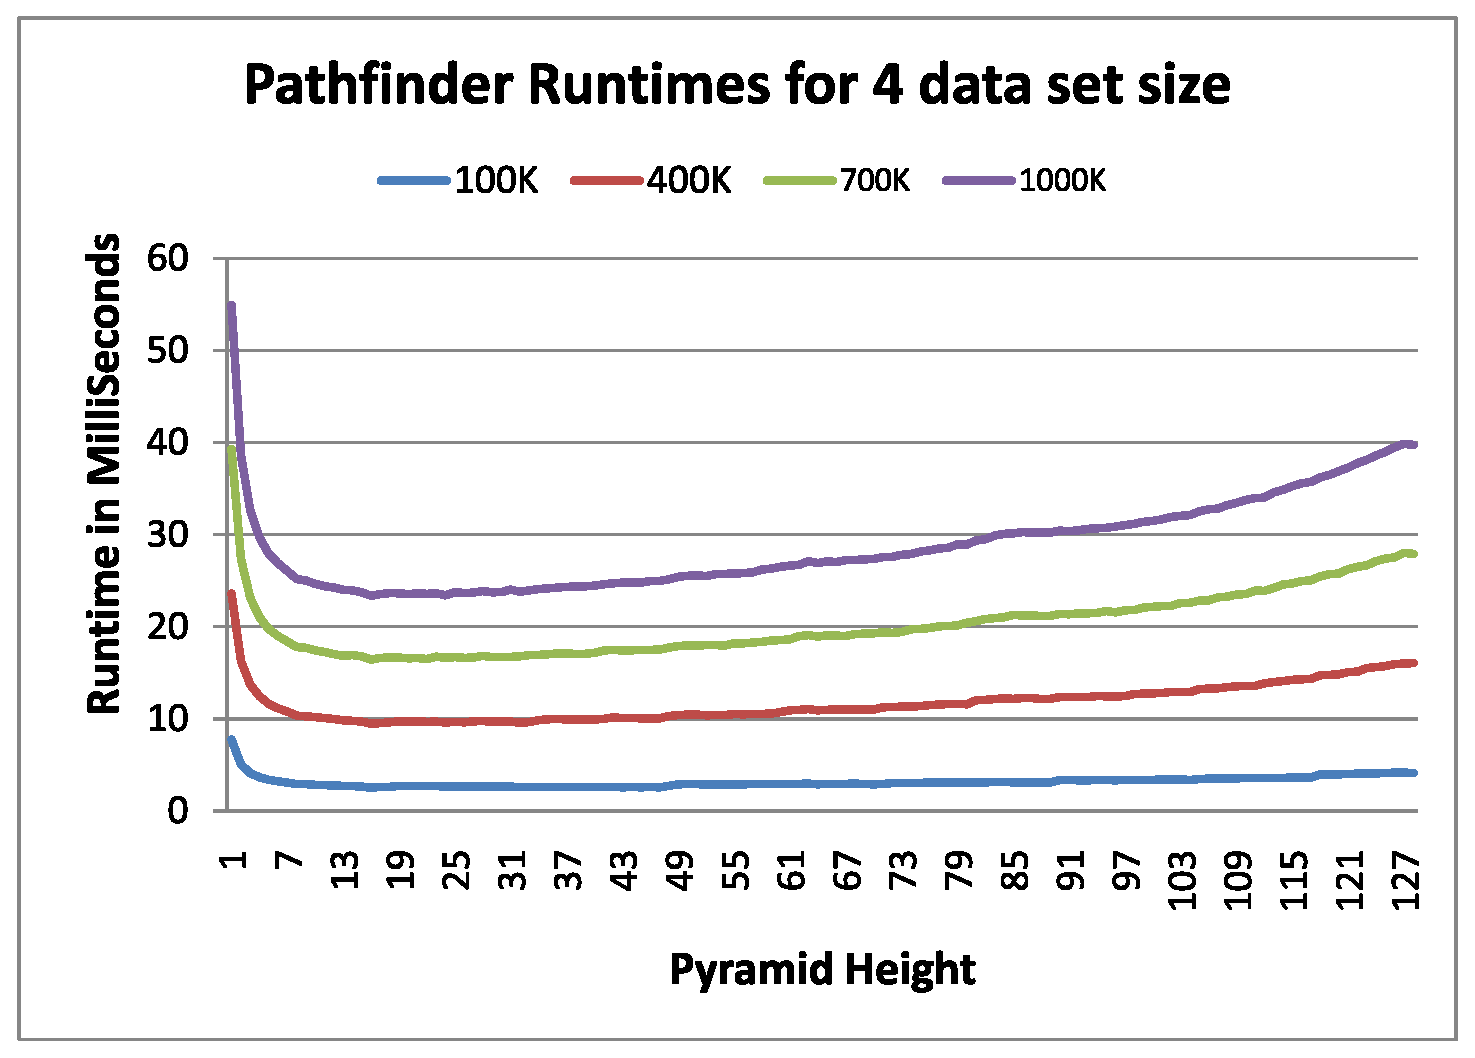
\includegraphics[clip,trim=1in 1in 1in 1in,width=3.3in]{figures/PathfinderTimingData}
\caption{Runtimes for the Pathfinder 1D application vs. PH.
The lowest portion of the curves are very flat.  Therefore, even though our model did not 
pick the best PH for any data set size, the performance was within 0.99\% and 2.79\% of optimal.}
\label{fig:pathfinderTimes}
\end{figure}

\subsection{\em ``Hotspot''}
The second test case is a 2D stencil application called {\em ``Hotspot''}.  
The stencil language description for this application is shown in Figure~\ref{fig:hotspot}.
The application calculates an ordinary differential equation that models heat dissipation in a conductive material.  
In this case, the modeled material is the silicon substrate of a computer chip~\cite{hotspot}.
On each time step of the computation, the heat generated by the chip components are injected through the modeled substrate.  
This is constant read-only data read for each cell on each iteration.  As this is a 2D application, 
the theoretical maximum square tile size on a GT200 card is 22x22.
This implies a possible PHs range from 1 to 10.  The resultant runtimes vs. PH are show in
Figure~\ref{fig:hotspotTimes}.  As can be seen, for the four data set sizes, the optimal PH is 2.
That is also the height calculated by our optimizer.  
\begin{figure}
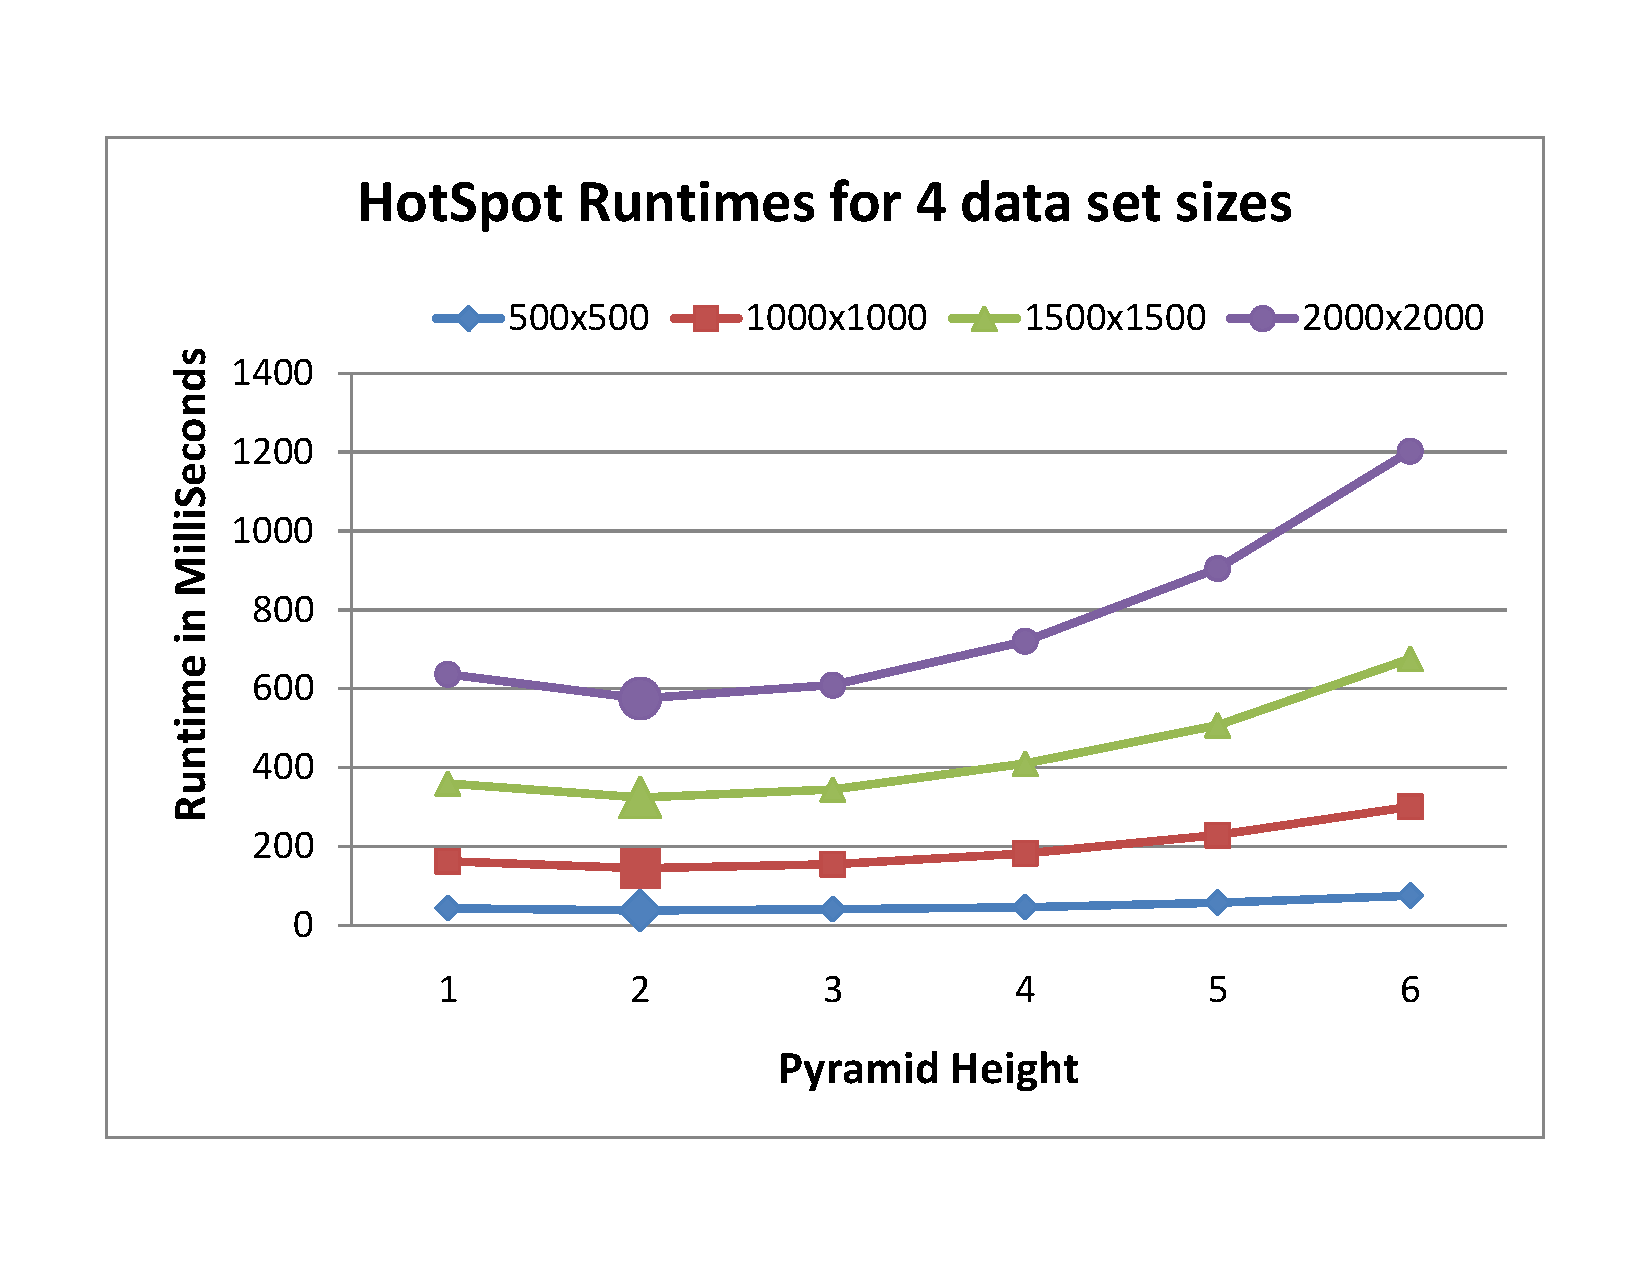
\includegraphics[clip,trim=1in 1in 1in 1in,width=3.3in]{figures/HotSpotTimingData}
\caption{Runtimes for the Hotspot 2D stencil application vs. PH.
As can be seen, the curve is bowl shape with a noticeable low point at PH 2.  The effect is more pronounced
with greater data set sizes.  Our optimizer picked the correct PH of 2 for all these data sets.}
\label{fig:hotspotTimes}
\end{figure}

\subsection{\em ``Plate''}
The third test case is another 2D stencil application called {\em ``Plate''}.  
It is very similar to and replaces the {\em ``Poisson''} application from the original test suite.  
It also models heat transfer in a plate but this time, the heat 
injection into the system is modeled as coming from the edge of the plate, not distributed throughout the plate.  
The makes the application different from Hotspot in two important ways.  
First, there is no required read of global data in each time step.  
Second, it gave us an opportunity to use the {\bf EdgeValue} capability of 
the SL to inject the heat at the plate's edge.  
Again the maximum square tile size on a GT200 card is 22x22 and valid PHs are 1 through 10.  
Again both the optimal PH and our model's predicted PH is 2 for all four data set sizes.
As the results for Plate are so similar to Hotspot, we don't include a graph.

\subsection{\em ``Cell''}
The fourth test case is a 3D stencil application called {\em ``Cell''}.  It models Conway's Game of Life in 3 dimensions.  
In each time step, each cell calculates whether it is alive or dead based on the number of neighboring cells that were alive in the previous
time step.  To perform this calculation, it looks at its 26 nearest neighbors.  
For a 3D application, the maximum tile size on a GT200 card is 8x8x8, 
and the possible PHs are only 1 to 3.  The runtimes vs. PH are shown in Figure~\ref{fig:cellTimes}.  
It is very clear from the chart that a PH of 3 is a very bad choice.  The runtimes for PHs of 1 and 2 are similar, 
but 1 is better and is also predicted by our model.
\begin{figure}
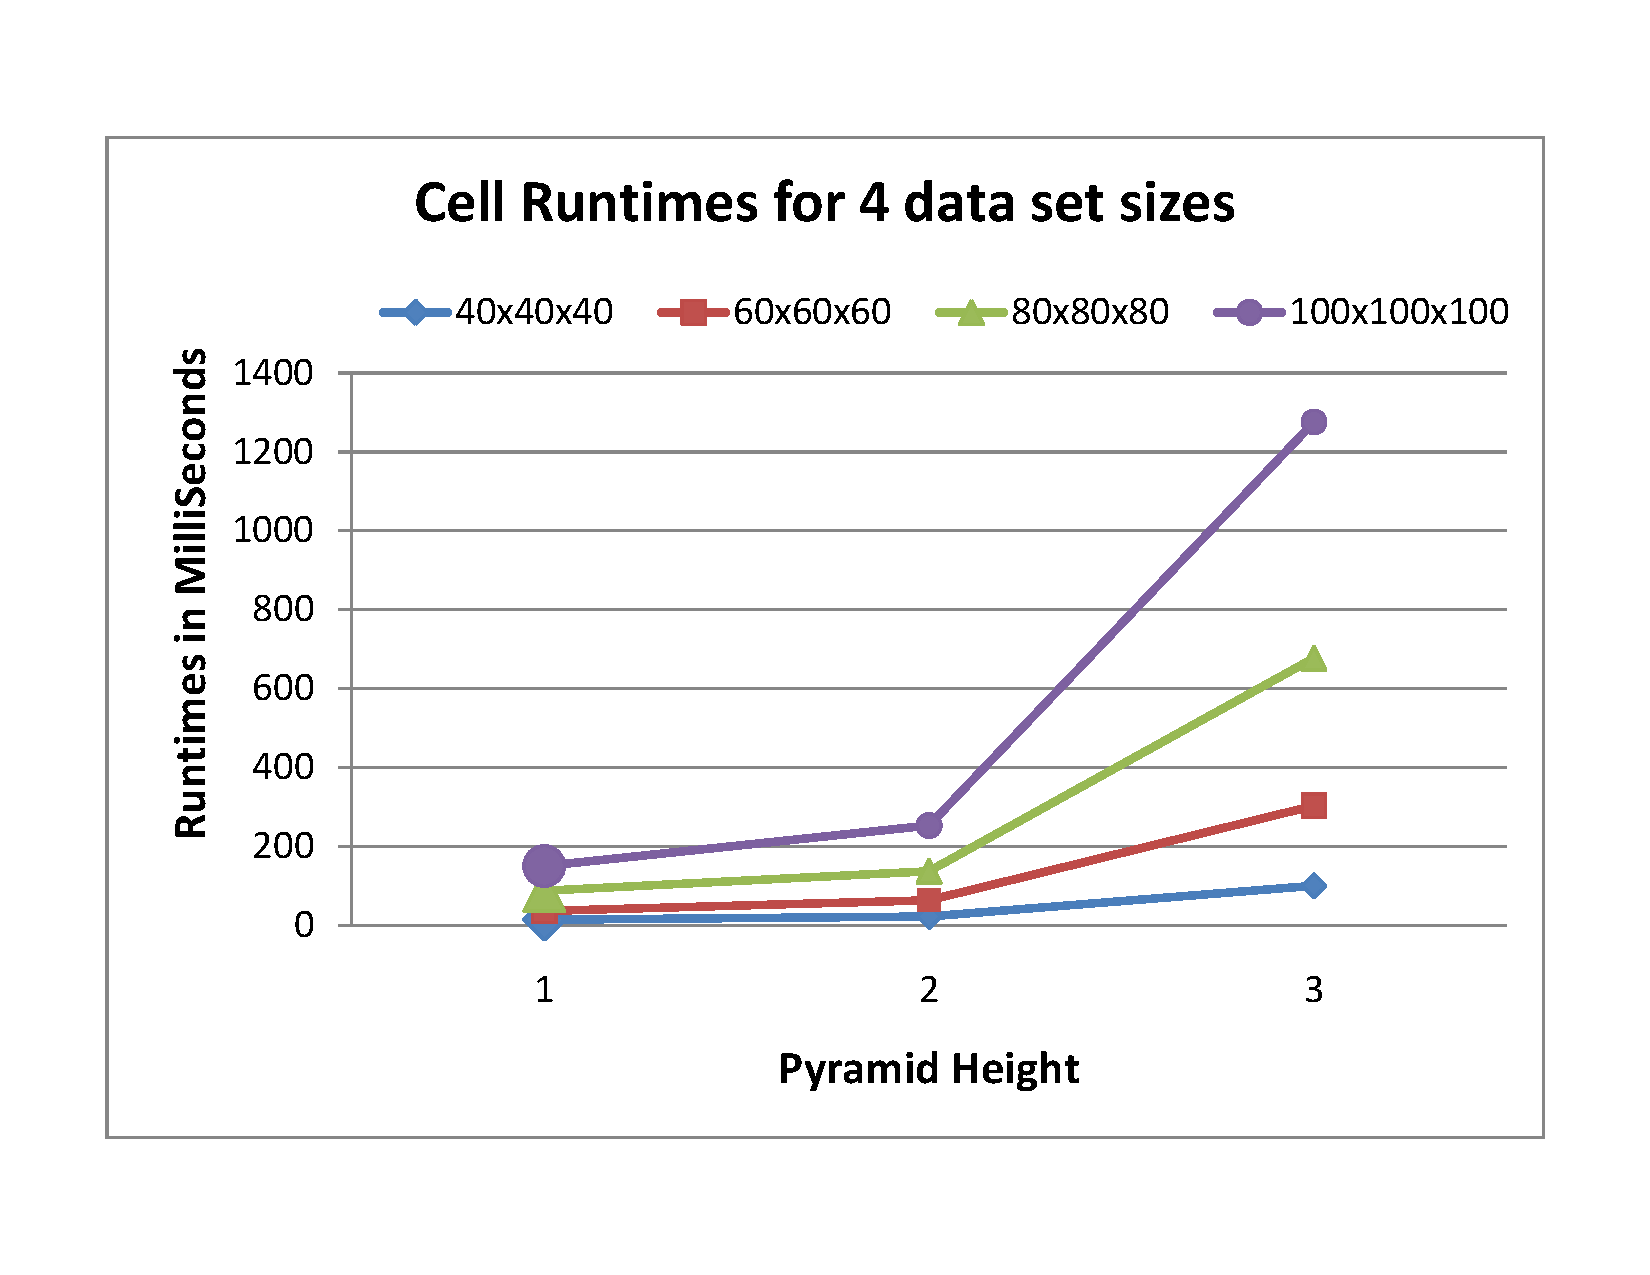
\includegraphics[clip,trim=1in 1in 1in 1in,width=3.3in]{figures/CellTimingData}
\caption{Runtimes for the Cell 3D stencil application vs. PH.
The curve shows that a PH of 3 is a very bad choice.  While the values for 1 and 2 are slightly 
compressed in the graph the optimal PH is in fact 1 for all data sets, as was accurately predicted by our optimizer.}
\label{fig:cellTimes}
\end{figure}

\subsection{Model Comparisons}
As we have demonstrated, our model predicts the optimal PH for 
Hotspot, Plate, and Cell on the GTX-280 card.
These were the same PHs predicted by the original model of Meng and Skadron 
for these same applications and data set sizes.  However, they
measured an optimal PH of 3 for Hotspot and Poisson.  
Their application implementations differ from ours in two important ways.  

First, as their applications were hand optimized, they were able to load the
read-only heat data used in Hotspot into shared memory to take advantage of
temporal locality.  Our SL has no way for the application programmer to express
the access patterns for read-only data, and therefore our version of Hotspot
will read the value from global memory in each time step.  The ability of the
hand optimized code to reuse the global memory read across several time steps
tends to drive the optimal PH higher, leading to greater temporal reuse
of data values loaded into shared memory.
We hope to add better support for read-only data to SL at a future date.

Second, their inner loop code calculates the cell values for all cells in the
tile, even those that have become too far away from the center of the tile to
matter to the computation.  Another option is to recalculate the zone of cells
involved in useful computation on each time step.  This keeps threads from
calculating values that will never be used at the cost of more GZ size
calculations.  Given that our system must access read-only data from global
memory in Hotspot (and potentially in other apps), the strategy of
recalculating the GZ size in each time interval mitigates the number of global
reads required, and is therefore the correct choice for such applications.

We found that 2D and 3D applications run faster by restricting the number of
calculated values, even without using read only data. We believe this is
because whole thread warps on the top and bottom of the tile will only have to
check on each time step if they are still calculating useful values.  In 3D
apps, this effect is even more pronounced as thread warps in the front and back
of the tile have this same advantage.  The GZs on the sides of the tile tend
not to span entire warps, so there is no advantage for warps at the sides of
the tile from this effect.  And the GZs in a 1D app only grow on the sides.
Our CUDA templates take advantage of these effects by continuing to calculate
values in the GZ for 1D stencil applications, but not for 2D or 3D
applications.  As a result of this change, our Pathfinder runtimes were
significantly reduced.

\begin{figure}
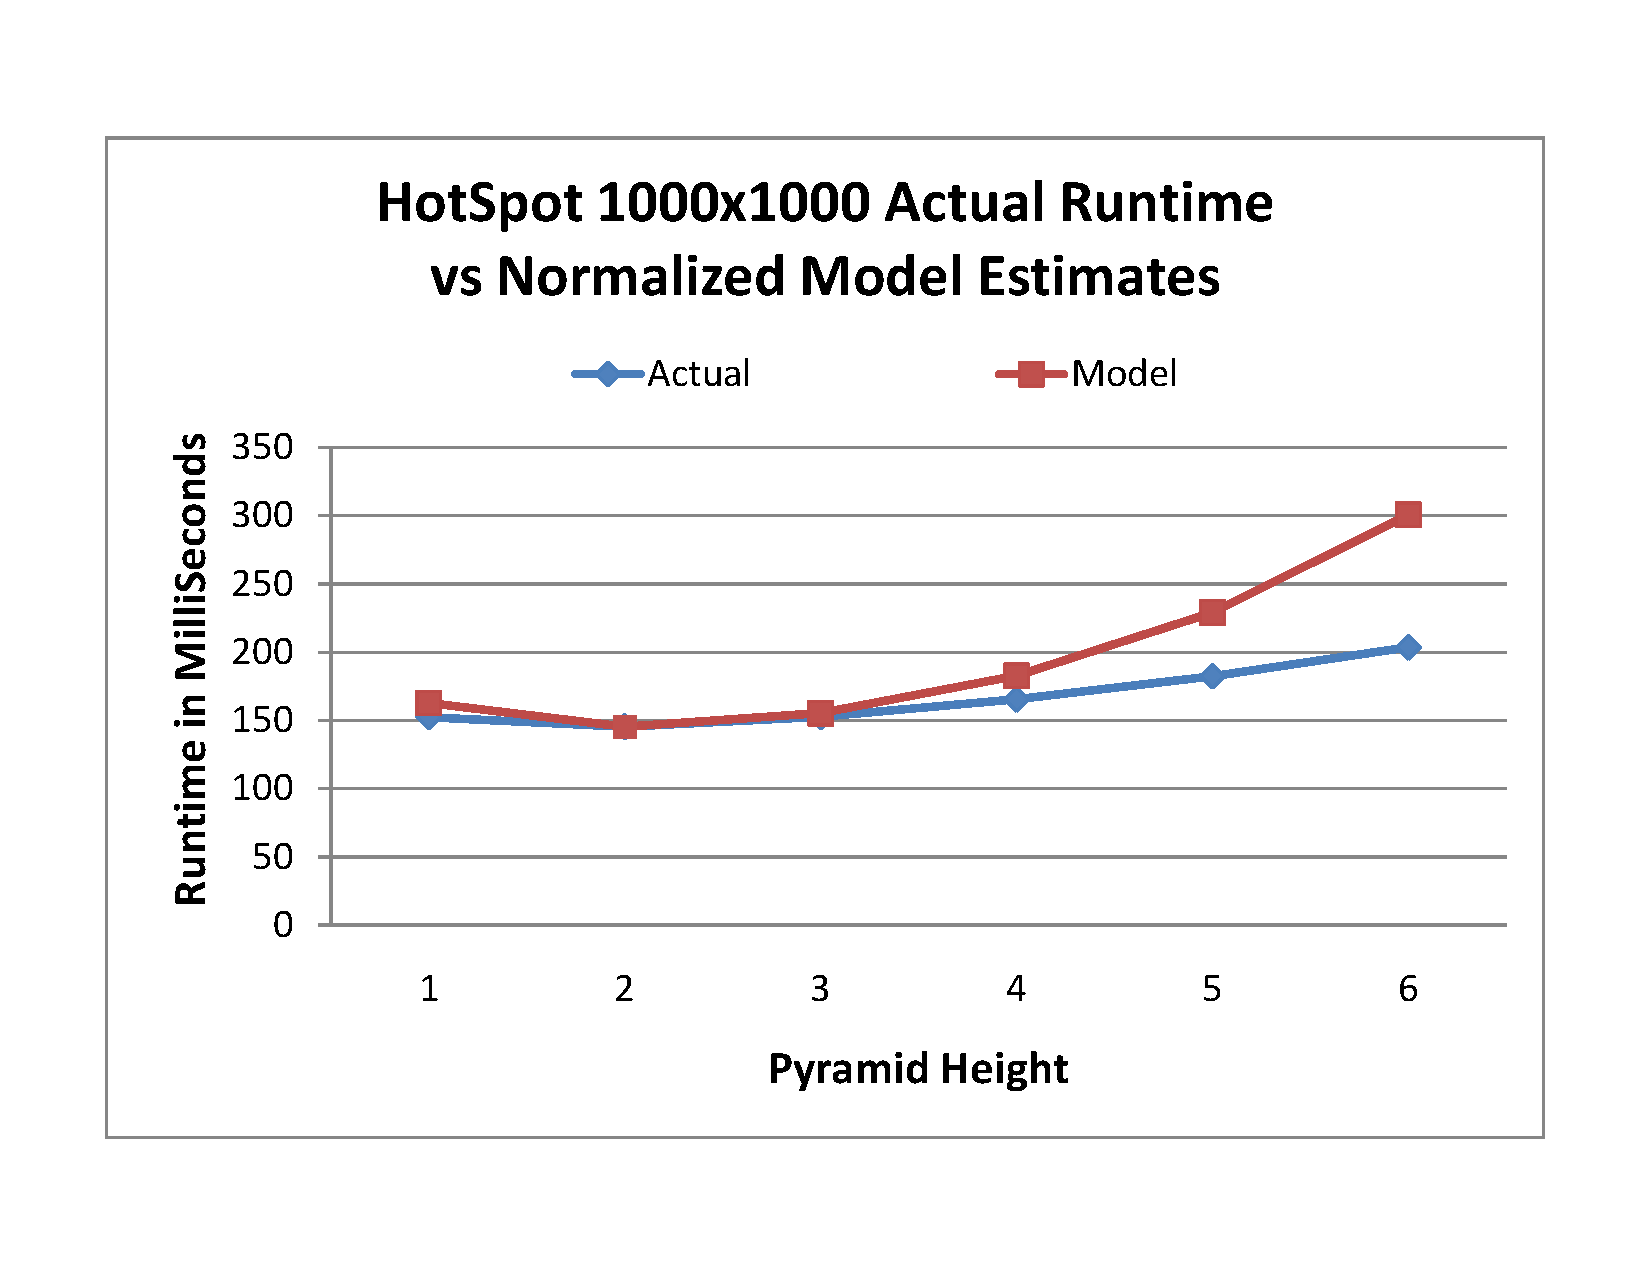
\includegraphics[clip,trim=1in 1in 1in 1in,width=3.3in]{figures/HotSpotModelActual}
\caption{
Runtimes for Hotspot vs. normalized runtimes predicted 
by the Model for PHs from 1 to 6.  
While the shape of the model curve does not exactly match the measured runtimes,
the model accurately predicts an optimal PH of two.
}
\label{fig:modelvsactual}
\end{figure}

We also analyzed the actual runtimes vs. our model predictions.  
Figure~\ref{fig:modelvsactual} shows Hotspot runtimes vs. predictions for 
PHs from 1 to 6.  
The model predictions are in terms of GPU cycles, not runtimes.  
Therefore, the model times are normalized to the actual runtime at the optimal PH=2.
This allows a more direct comparison of the relative curves shapes, which is
more important than absolute scaling for choosing the optimal PH.
As the figure shows, the model has a steeper bowl shape
than the actual runtimes.  The effect is more pronounced for higher PHs, and really grow large quickly for PHs 
between 6 and 10.
% which were truncated to better show the most interesting part of the curve.

The results presented here validate that the changes that we have made to the 
CUDA ISL analytical model have not lessened the effective accuracy of its PH predictions.
Given the advantage of the elimination of the users' manual involvement in this 
optimization, we believe this to be an important contribution of this work.

\subsection{Comparison to Na\"{i}ve CUDA code}

\begin{table*}
\centering
%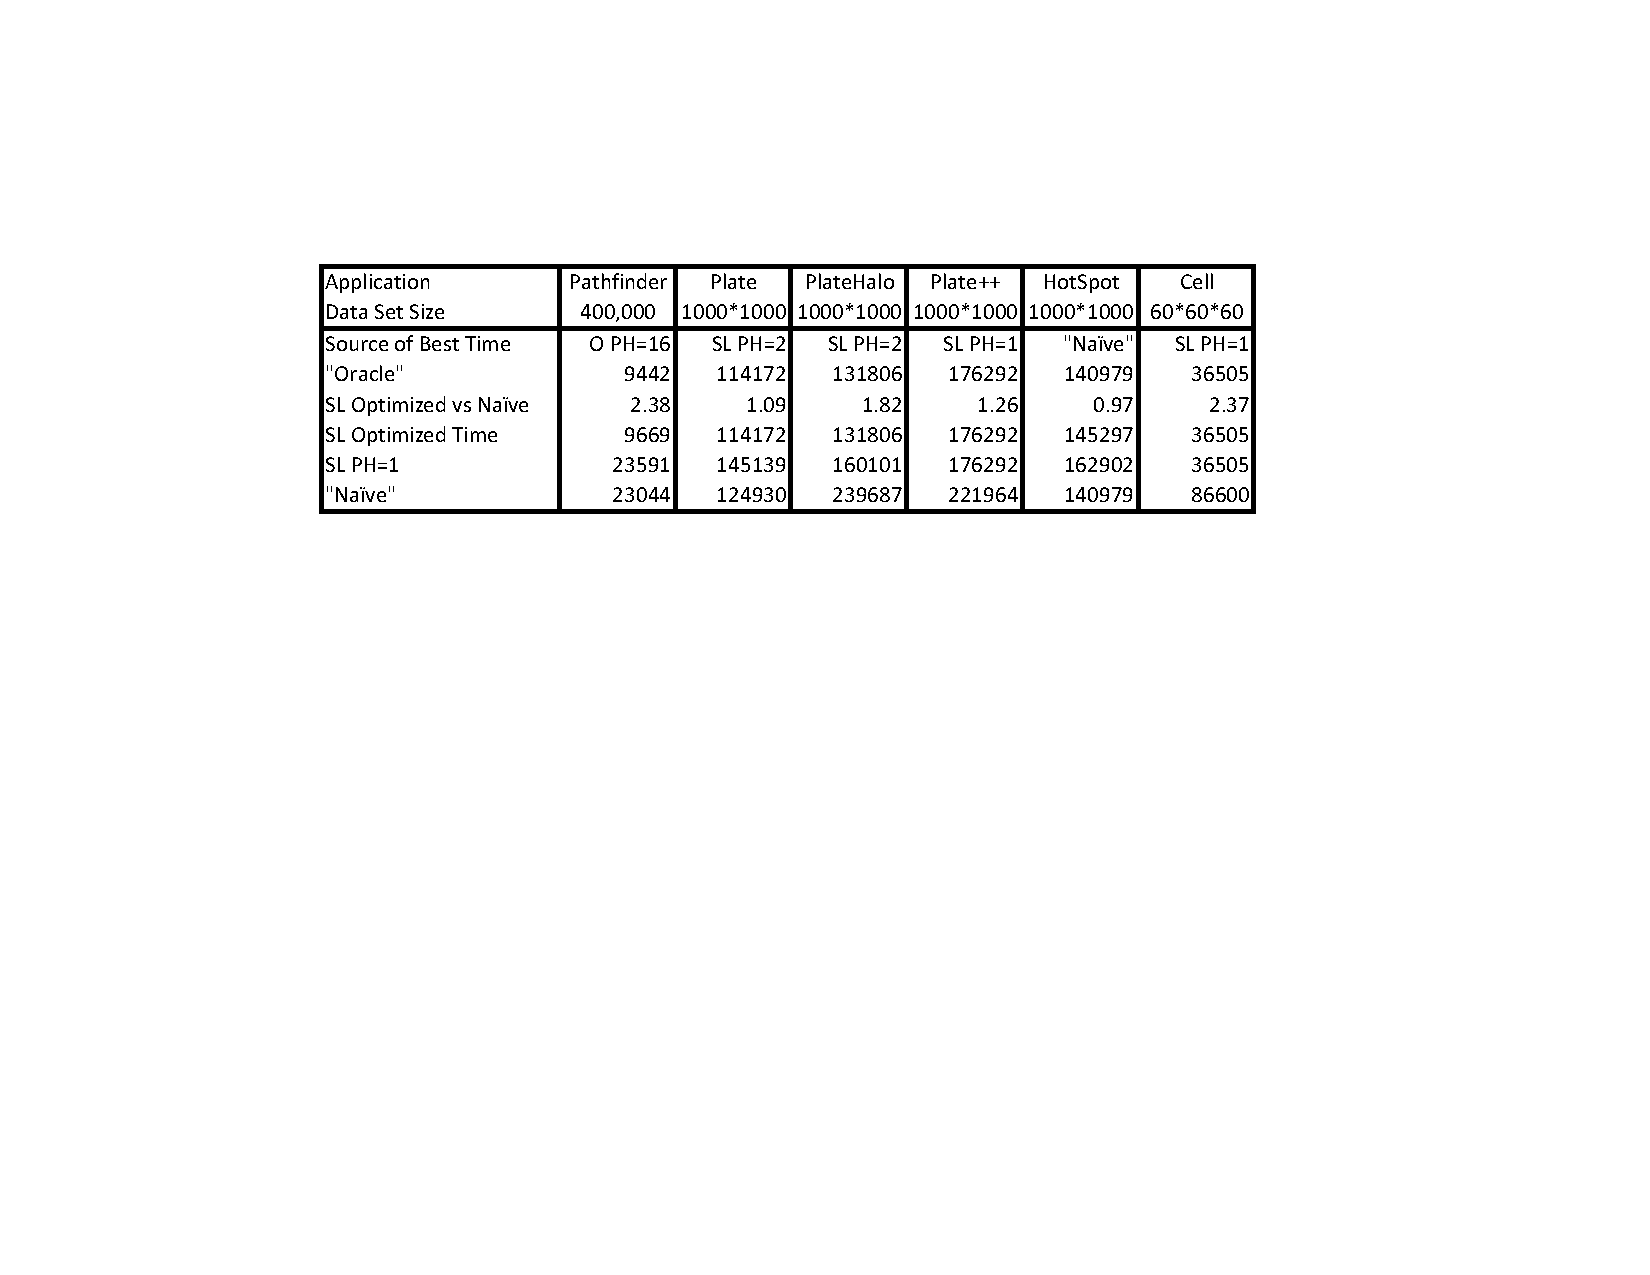
\includegraphics[clip,trim=2in 5in 2.4in 1.7in,width=4.5in]{figures/GT200Table}
\begin{tabular}{|l|c|c|c|c|c|c|}
\hline
{\bf Application} & {\bf Pathfinder} & {\bf Plate} & {\bf PlateHalo} & {\bf Plate++} & {\bf Hotspot} & {\bf Cell} \\
Data Set Size	& 400K	& $1000^2$	& $1000^2$	& $1000^2$	& $1000^2$	& $60^3$	\\
\hline
Source of Best Time & O PH=16 	& SL PH=2	& SL PH=2	& SL PH=1	& Na\"{i}ve	& SL PH=1	\\
Oracle		& 9442 $\mu$s	& 114172 $\mu$s	& 131806 $\mu$s	& 176292 $\mu$s	& 140979 $\mu$s	& 36505 $\mu$s	\\
SL Optimized vs Na\"{i}ve & 2.37 & 1.09		& 1.82		& 1.26		& 0.97		& 2.37		\\
SL Optimized Time & 9716 $\mu$s	& 114172 $\mu$s	& 131806 $\mu$s	& 176292 $\mu$s	& 145297 $\mu$s	& 36505	$\mu$s	\\
SL PH=1		& 23591	$\mu$s	& 145139 $\mu$s	& 160101 $\mu$s	& 176292 $\mu$s	& 162902 $\mu$s	& 36505	$\mu$s	\\
Na\"{i}ve	& 23044	$\mu$s	& 124930 $\mu$s	& 239687 $\mu$s	& 221964 $\mu$s	& 140979 $\mu$s	& 86600	$\mu$s	\\
\hline
\end{tabular}
\caption{
Runtimes for the SL optimized code for the four applications in Section 7, plus
two new versions of Plate.  Runtimes are also shown for a na\"{i}ve CUDA
implementation, along with a comparison relative to SL optimized code.  For
applications with large amounts of either temporal or spatial locality, the SL
generated code far outperforms the na\"{i}ve code.  For other applications, the
difference is more modest.
}
\label{fig:GT200Table}
\end{table*}

\begin{table*}
\centering
%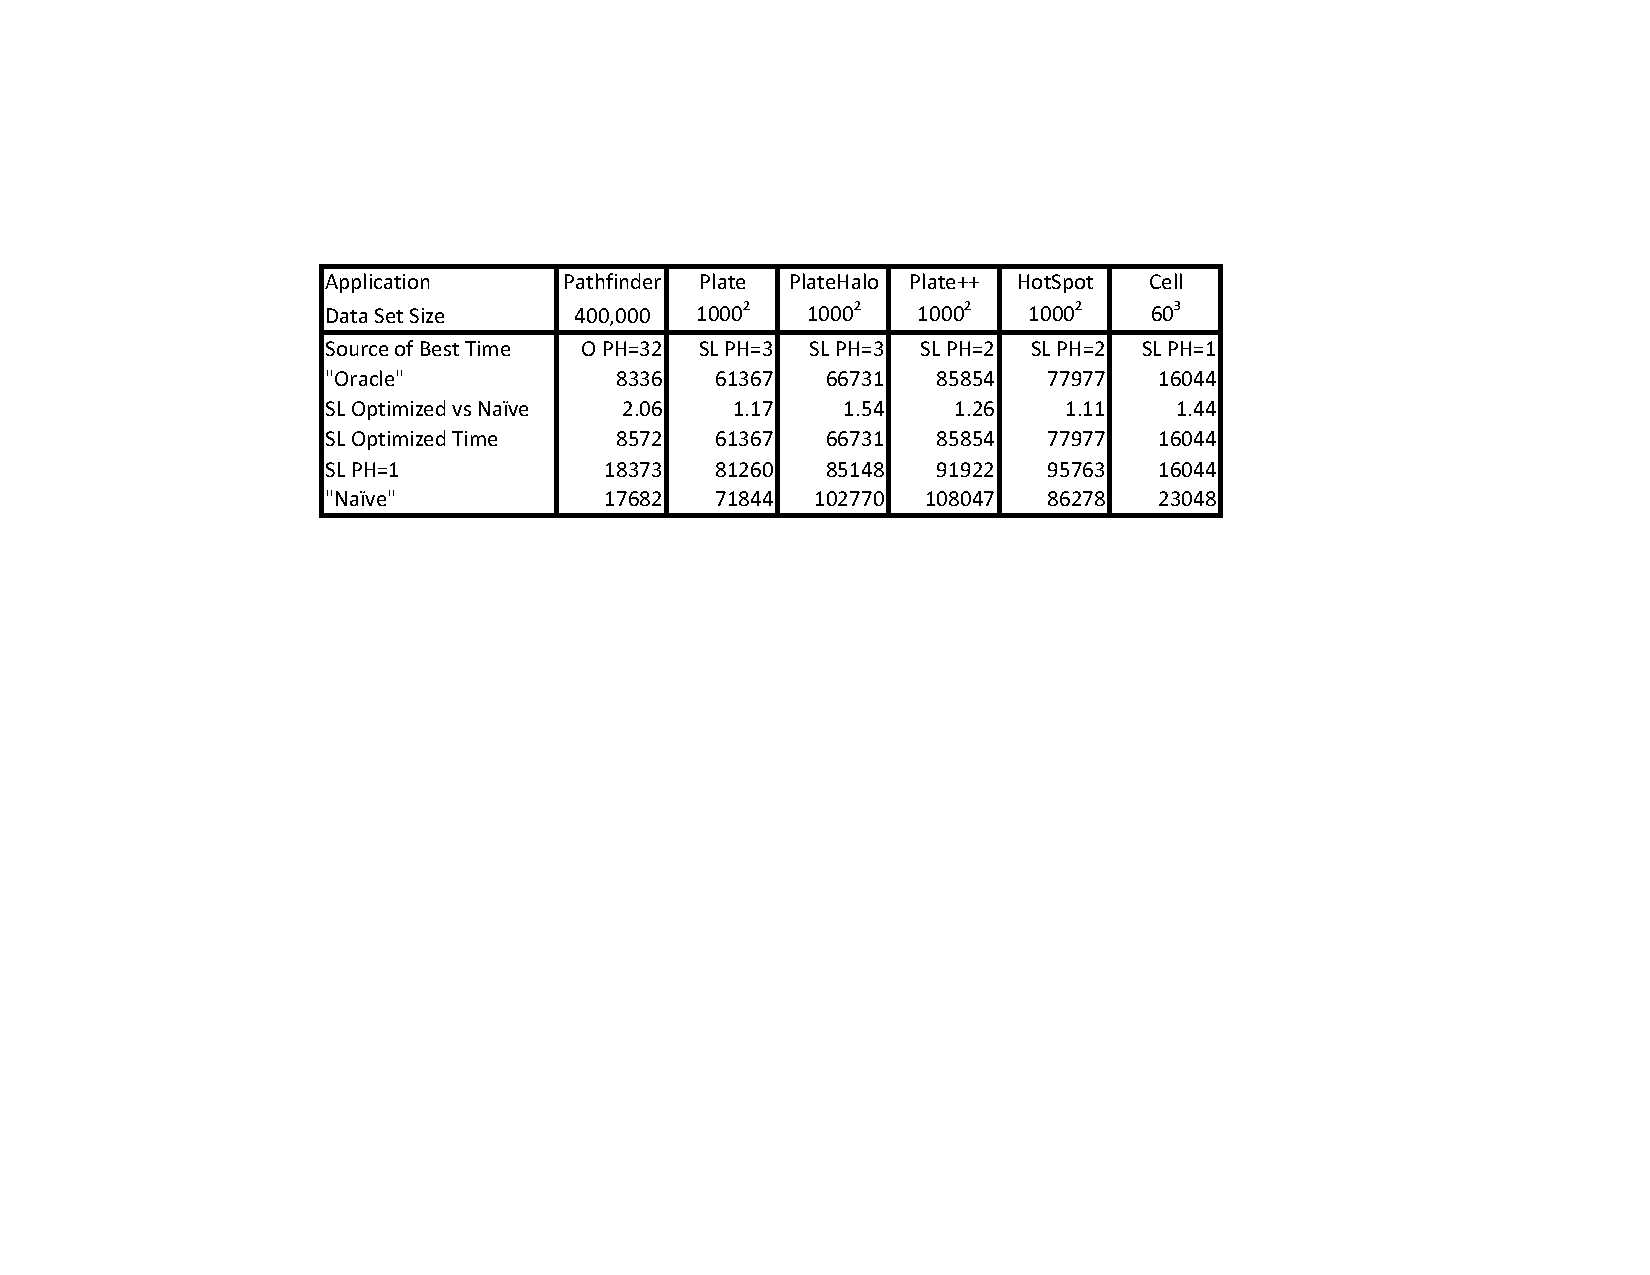
\includegraphics[clip,trim=2in 5in 2.4in 1.7in,width=4.5in]{figures/FermiTable}
\begin{tabular}{|l|c|c|c|c|c|c|}
\hline
{\bf Application} & {\bf Pathfinder} & {\bf Plate} & {\bf PlateHalo} & {\bf Plate++} & {\bf Hotspot} & {\bf Cell} \\
Data Set Size	& 400K	& $1000^2$	& $1000^2$	& $1000^2$	& $1000^2$	& $60^3$	\\
\hline
Source of Best Time & O PH=32 	& SL PH=3	& SL PH=3	& SL PH=2	& SL PH=2	& SL PH=1	\\
Oracle		& 8336 $\mu$s	& 61367 $\mu$s	& 66731 $\mu$s	& 85854 $\mu$s	& 77977	$\mu$s	& 16044 $\mu$s	\\
SL Optimized vs Na\"{i}ve & 2.06 & 1.17		& 1.54		& 1.26		& 1.11		& 1.44		\\
SL Optimized Time & 8572 $\mu$s	& 61367	$\mu$s	& 66731	$\mu$s	& 85854	$\mu$s	& 77977	$\mu$s	& 16044	$\mu$s	\\
SL PH=1		& 18373	$\mu$s	& 81260	$\mu$s	& 85148	$\mu$s	& 91922	$\mu$s	& 95763	$\mu$s	& 16044	$\mu$s	\\
Na\"{i}ve	& 17682	$\mu$s	& 71844	$\mu$s	& 102770 $\mu$s	& 108047 $\mu$s	& 86278	$\mu$s	& 23048	$\mu$s	\\
\hline
\end{tabular}
\caption{
Data similar to Table~\ref{fig:GT200Table} but now run on the Fermi series
GTX-480 GPU card.  Note that the increased block size on Fermi results in
higher optimal PH for Plate, PlateHalo, and Plate++ due to the larger tile
sizes.  The inclusion of a cache on Fermi also results in a lower relative
improvement of SL optimized code vs na\"{i}ve for applications with large
amounts of temporal or spatial locality.
}
\label{fig:FermiTable}
\end{table*}

In judging the performance of optimized code, it is important to
see the effects of the optimizations compared against code that
does not have those optimizations.  Table~\ref{fig:GT200Table}
shows where we compare a ``na\"{i}ve'' CUDA 
implementation for the four applications discussed above along
with two additional applications.  

The na\"{i}ve CUDA implementation does not use shared memory.
Instead, global device memory is always accessed.
Therefore, each PE can only calculate one time step 
before synchronizing with neighboring PEs.
While there are some edge cases to consider at the
boundaries of the data set, there is no longer any
need to handle edge cases across internal tile boundaries.
However, the na\"{i}ve code does still benefit from
large tile sizes, and the maximum possible size is used.
Overall, this code is much simpler than the optimized code,
and would presumably be easier to write by hand.

Table~\ref{fig:GT200Table} also shows the runtimes of
the SL generated code, but with PH=1.  Finally,
the table also shows the runtime of the SL generated code with
an ``oracle'' picking the best code.  This often matches the SL
optimized code, but differs in those cases where
SL does not accurately predict the best PH, and the one
case where the na\"{i}ve code outperforms the SL 
generated code.

We can see from the table that the SL generated code outperforms the na\"{i}ve
code by between 2.37X and 0.97X with an arithmetic mean of 1.65X.
The SL optimized code outperforms the na\"{i}ve code by a significant factor
for both the 1D Pathfinder application, and the 3D Cell application, but for
different reasons.  In Pathfinder, the optimal PH is high at 16, so there is
substantial temporal reuse of the data values stored in shared memory even
though the spatial reuse is limited by the single dimension of the data.  This
is further seen by looking at the PH=1 runtime for the SL code.  By setting the
PH=1, all of the temporal reuse is eliminated, and the overhead of the
additional complexity of the SL code causes it to run slightly slower than the
na\"{i}ve code.

On the other hand, in Cell, the stencil involves 26 neighboring cell values.
So, even though the temporal reuse is non-existent with an optimal PH of 1, 
the spatial reuse is significant.
In the 2D applications, the optimal PH of Plate and Hotspot
on the GTX-280 are both 2, and the stencil involves 4 adjacent cells.  
So neither the spatial nor temporal reuse is extremely high.
In fact the na\"{i}ve code runs faster than SL's optimal
code for Hotspot, as the latter is also doing global memory reads
in each time step.

To further explore these issues, we added two additional versions of Plate
to our study.  The first -- called {\em PlateHalo} -- expands the number of
adjacent cells used in the computation to 8 by including the diagonal
neighbors.  This increases the spatial locality of the data in shared
memory, and we see that the runtime for the na\"{i}ve version almost doubles
in PlateHalo over Plate, where the SL optimized version only slows by 15\%.  
The SL optimized version of PlateHalo outperforms the na\"{i}ve version by 1.8X.

The second variation of Plate is called {\em Plate++}.  It also
expands the stencil to include 8 neighbors, but this time by going out 2 cells
to the north, south, east, and west.  As this causes the GZs to grow twice as
fast as in Plate, the optimal PH is now 1.  So, temporal reuse is eliminated in
the SL code, and SL code for Plate++ runs slower than either Plate or
PlateHalo.  The na\"{i}ve code for Plate++ runs 8\% faster than the na\"{i}ve
code for PlateHalo perhaps because of better memory access coalescence, or fewer
memory bank conflicts.

\subsection{Fermi Results}

We reran the tests from Table~\ref{fig:GT200Table} on a GTX-480, a Fermi series
GPU.  This machine contains a Core 2 Q9400 running at
2.66GHz with 6MB of L2 cache, and 5GB of DRAM.  The system installation was
otherwise identical to the GT200.  On Fermi cards, the maximum
threads per block is expanded to 1024, with 60 PEs each with 8 SIMD cores.  The
GTX-480 runs at 1.4GHz, and has a small global memory cache.  The test results are
shown in Table~\ref{fig:FermiTable}.

The increased numbers of threads per block means that the tile sizes for all
applications are raised.  As a result, the optimal PH for the applications
tends to be higher because the GZ size for a given PH is a smaller percentage
of the tile size.  The optimal PH for Plate and PlateHalo have increased from 2
to 3, and for Plate++ is has increased from 1 to 2.  For the shown data sizes,
SL properly predicted these changes in optimal PH.  However, for some of the
other data set sizes SL did not.  The worst prediction is for Cell with a data
set size of 40*40*40 with a resultant slowdown of 83\%.  The next worse was
only 11\%.  The arithmetic mean of the slowdown over all tested applications
and data set sizes was only 4.7\%.

The inclusion of a cache on Fermi cards results in a reduction in the relative
advantage of using the scratchpad memory for temporal and spatial
locality.  We see this in the reduced advantage of the SL optimized code
over na\"{i}ve in the 1D, 3D, and PlateHalo applications where these
effects were largest on the GT200 architecture.  Still, the SL optimized code
performs better than the na\"{i}ve code by between 2X and 1.1X with an
arithmetic mean of 1.43X.

\section{Related Work}

Li et al. may have been the first to use the term
{\em iterative stencil loops}~\cite{li}.  They developed a compiler
framework for these loops that used tiling to improve temporal data
locality.  Their work was intended to be run on a uniprocessor, so
they did not face any communication costs and they did not consider
ghost zones.

We are not the first to create a stencil compiler.  Brickner et al.
created a stencil compiler for the Connection Machine CM-2 massively
parallel architecture~\cite{cm2}.  The stencil expression was
expressed in ``microcode'' which was specific to
the CM-2.

In parallel with our efforts, Orchard et al.~\cite{ypnos} have developed a
stencil language called {\em Ypnos} as an extension to Haskell.  They also argue for an
architecture-independent declarative language for ISLs, and as in SL rely on language
features instead of complex program analysis to determine the size and shape of
the stencils and data.  Their language includes reduction operators as a means
for specifying convergence criteria, and they allow users to explicitly specify
a PH for an ISL computation, but do not support automatic PH optimization.
They do not report Ypnos performance results.  Finally, our users specify
the CellValue and EdgeValue calculations in C, as we feel it is more
widely-accessible than Haskell. 

Kamil et al.~\cite{kamil} studied the effects of tile size and time skewing to
increase memory locality on the Itanium2, Opteron, Power5, and Cell.  They
concluded that controlling tile size, temporal locality across time slices, and
hand-tuned control of scratchpad memory is critical to performance.  We
optimize use of CUDA's scratchpad memory, tile size, and temporal reuse.
However, our temporal locality is always strictly in the time dimension; we
have not investigated use of time skewing.  Datta et al.~\cite{AutoTuning}
studied optimizations for stencil applications across a wide range of
architectures including CUDA.  However, their optimizer uses auto-tuning to
find optimal solutions.  Our analytical model starting point allows our
training period to be very short relative to a typical ISL computation.

Micikevicius explored hand coding stencil applications on CUDA, and 
ghost zone sizes~\cite{Micikevicius}.  They also
explored using asynchronous data transfers for data sets too large to fit
in GPU global memory.  Volkov et al. explored
hand optimizing CUDA programs involving parallel operations on large
arrays~\cite{volkov}.  We have included a subset of the optimizations presented
by Micikevicius and Volkov in our CUDA template library,  but we have no
support for arrays too large to fit into the devices global memory, and
therefore we did not investigate asynchronous data transfers.

Several attempts have been made to build simplifying layers on top of
the CUDA language.  Lee et al. built a source-to-source
translator for OpenMP to CUDA~\cite{openmp2gpu}.  
OpenMP can express a significantly wider range of parallel computations then that
which can be expressed by SL.  However, this also
means an OpenMP translator cannot include stencil application specific
optimizations as we do.

CUDA-lite is a general purpose source-to-source translator for automatically
optimizing CUDA programs~\cite{cudalite}.  The user specifies a na\"{i}ve CUDA
implementation of their ISL that only uses global memory, and adds some pragmas
that give hints about the size, shape, and data access patterns.  Then
CUDA-lite generates an optimized CUDA program that leverages the
specialized memory spaces, resulting in 2-17X speedups for their test
applications.  It appears they ran their tests on earlier GPUs that had much
less flexible memory access coalescing hardware than modern GPUs.  In addition,
their primary test applications were not stencil applications, and instead
performed operations such as matrix multiply. These contain large amounts of
spatial and temporal locality, and are compute intensive, allowing for more
processing time to hide memory access latency~\cite{Ryoo}. By comparison, SL
also optimizes for shared memory but not texture memory, and also
optimizes PH.

\section{Conclusions and Future Directions}

We have defined a new language, SL, for easily expressing stencil applications.
SL is a formal high-level language in which a programmer can conveniently
describe an ISL computation by focusing on the simple computation needed to
compute cell values.  No optimization nor architectural-specific information is
needed.

We have created a SL compiler that uses templates to allow the generated code
to be extended to many parallel execution environments.  Based on a single
source file, it could output efficient code for CUDA, OpenCL, OpenMP, pthreads,
or other environments.

We have implemented an initial template and an optimizer for the CUDA
programming environment that blocks computations to use the scratchpad memory,
and that estimates the best PH.  The optimizer is fully automatic and utilizes
both static and dynamic application information.  It accurately
calculates the optimal tile size and PHs for several test applications, on both
GT200 and Fermi series GPUs.  As a result, with an SL declaration of
about 16 lines, a user can achieve average speedups of 1.65X\% for
the GTX-280, and 1.43X for the GTX-480, over na\"{i}ve CUDA code.
Yet the SL specification is much easier to write than even the
na\"{i}ve CUDA code, and is similar to writing code for a single
thread CPU.

The optimizer's ability to leverage
dynamically acquired information about the runtime environment
means that the generated code can be used on a variety of devices.
Our model ported directly from the GT200 architecture to
the next generation Fermi architecture with only trivial
modification.

The current SL architecture can be extended in several directions.  First, with
language extensions, we can improve support for read-only data at least in the
common cases such as Hotspot where the array access pattern is
straightforward.  A second SL language extension could add support for 
reduction operators, and ISL termination based on a data convergence criteria.  
It would also be interesting to investigate data morphing as a way to improve cache
performance or reduce memory bank conflicts.  

%\acks

%Acknowledgments, if needed.

% We recommend abbrvnat bibliography style.

\addtolength{\itemsep}{-0.2\baselineskip}
\balance
\bibliographystyle{abbrvnat}
\bibliography{PPoPP-report}

\end{document}
